\documentclass{report}

% Pacotes para acentuação e formatação

\usepackage[utf8]{inputenc}
\usepackage[T1]{fontenc}
\usepackage[brazil]{babel}
\usepackage{setspace}    % Para espaçamento
\usepackage{lipsum}      % Texto de exemplo (remova se não precisar)
\usepackage{graphicx}
\usepackage{hyperref}
\usepackage{listings}
\renewcommand{\lstlistingname}{Código}


\begin{document}
	
	\begin{titlepage}
		
		\centering
		\vspace*{5cm} % Espaço do topo
		
		{\Huge\bfseries Estrutura de Dados I\par} % Título
		
		\vspace{0.5cm}
		{\Large 2025/2\par} % Ano
		
		\vfill
		{\large Nicolas Ramos Carreira\par} % Nome
		
		\vspace*{2cm}
	\end{titlepage}
	
	\tableofcontents
	\newpage
	
	\chapter{Intuito}
	
	O intuito deste documento é documentar o meu aprendizado da disciplina de estrutura de dados 1. Nesta disciplina começamos estudando sobre a linguagem C até entrar nas principais estruturas de dados. 
	
	\chapter{Fundamentos em C}
	\section{Sobre a linguagem C}
	A linguagem C é uma das linguagens de programação mais influentes e utilizadas da história da computação. Criada na década de 1970 por Dennis Ritchie nos laboratórios Bell, ela foi projetada para ser uma linguagem de propósito geral, eficiente e próxima do hardware, permitindo alto desempenho.
	
	C é considerada uma linguagem de médio nível, pois combina características de linguagens de baixo nível (como manipulação direta de memória) com recursos de alto nível (como funções e estruturas). Sua sintaxe influenciou muitas outras linguagens modernas, como C++, Java, Csharp e até mesmo Python em alguns aspectos.
	
	É amplamente usada em sistemas operacionais, softwares embarcados, drivers e aplicações que exigem alto desempenho. Além disso, aprender C é um ótimo ponto de partida para entender conceitos fundamentais de programação e arquitetura de computadores.
	\section{Estrutura de um programa em C}
		
	\begin{center}
		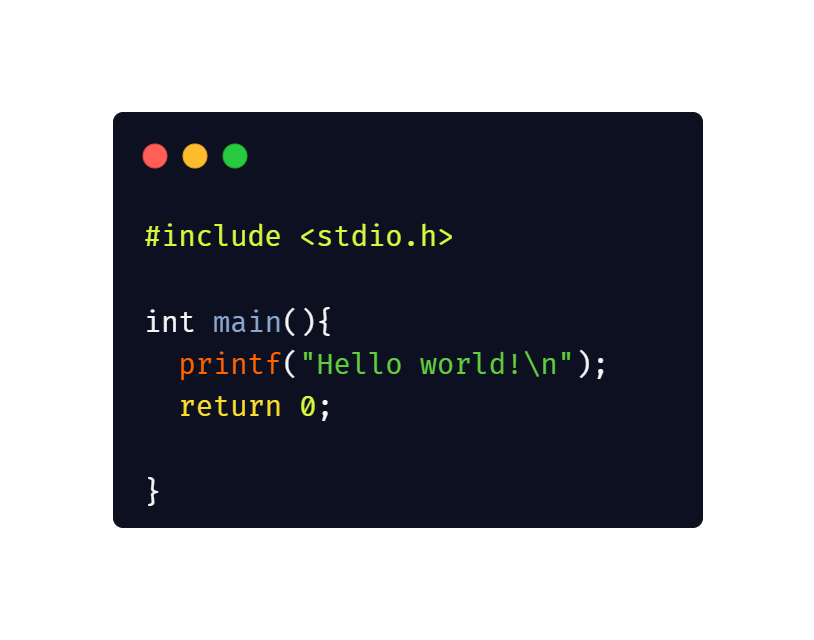
\includegraphics[width=6cm,height=5cm,keepaspectratio=false]{imagens/programac.png}
	\end{center}
	
	A imagem acima mostra um programinha extremamente simples em C, um Hello, world. Para iniciar um programa em C, nós sempre começamos declarando a biblioteca principal, que é a stdio.h (poderíamos ter outras bibliotecas inclusive, mas essa é a principal e DEVE estar lá). 
	
	Depois disso, nós declaramos o local do programa principal, onde fazemos o programa em si. 
	
	Um detalhe é que ao final de cada coisa SEMPRE temos que ter o ponto e vírgula (;), pois se não o nosso programa não compila.
	
	\section{Aspectos da linguagem C}
	\subsection{Variaveis}
	\subsubsection{O que são e pra que são usadas}
	Varivel, em linguagens de programação, é basicamente uma posição alocada da memória para guardar uma informação. Variaveis podem ser modificadas pelo programa e devem ser definidas antes de ser utilizadas
	\subsubsection{Declaração de variaveis em C}
    Para definir variaveis em C, nós precisamos passar o tipo de dado e nome da variavel, no formato: 
    
    \begin{LARGE}
    	\begin{center}
    		<tipo de dado> nome-da-variavel;
    		
    	\end{center}
    \end{LARGE}

    \begin{description}
     	\item[Obs:] ao fazer da forma acima, estamos apenas declarando a variavel, sem atribuir um valor a ela
     \end{description}
    
    O tipo de dado deve ser aqueles que são aceitos pela linguagem (inteiro, decimais, caracteres, booleanos..), mas como falaremos sobre tipos de dados mais pra frente, não entraremos em detalhes agora. O nome da variavel é algo bem importante a se considerar, pois existem algumas regras e boas práticas importantes quanto a isso:
    \begin{itemize}
    	\item Nomes de variaveis devem iniciar com letras ou underscore 
    	\item Os caracteres da variavel devem ser letras, numeros ou underscore (não utilizar acentos ou simbolos)
    	\item Não utilizar espaço em nomes de variaveis
    	\item Palavras chaves (palavras que são reservadas pela linguagem para fazer determinadas coisas) não podem ser usadas como nomes 
    	\item Letras maiusculas e minusculas são consideradas diferentes
    \end{itemize}
    
    Só para deixar totalmente claro, as palavras chaves que a linguagem C usa são:
    
    \begin{figure}[ht]
    	\centering
    	% ajusta a largura da imagem para ser quadrada (ex: 5cm x 5cm)
    	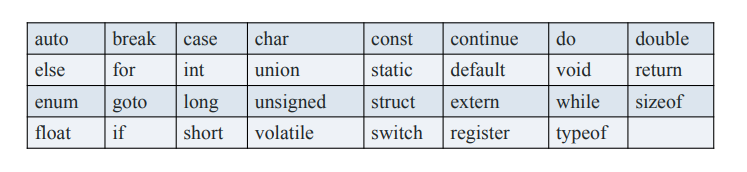
\includegraphics[width=9cm,height=2cm,keepaspectratio=false]{imagens/reservadas.png}
  
    \end{figure}
    
    \subsubsection{Atribuição de valores em variaveis}
    
    Tendo o formato <tipo de dado> nome-da-variavel, podemos atribuir valores a elas (ou seja, armazenar valores dentro da memória). Para isso, basta fazer:
    
    \begin{LARGE}
    	\begin{center}
    		<tipo de dados> nome-variavel = valor;
    	\end{center}
    \end{LARGE}
    
	\subsection{Tipos de dados}
	Como falamos anteriormente na parte de variaveis, quando vamos defini-las, nós temos que declarar o tipo de dado da variavel. O tipo de dado define os valores que aquela variavel pode assumir e as operações que podem ser realizadas com ela.
	Os tipos de dados principais são: char, int, float e double
	\subsubsection{Char}
	Um byte que armazena
	\subsubsection{Int}
	Um inteiro cujo o tamanho do numero que pode ser alcançado depende do processador (tipicamente 16 ou 32 bits)
	\subsubsection{Float}
	Basicamente numeros decimais com precisão simples (em C a parte decimal usa ponto e não vírgula)
	\subsubsection{Double}
	Também números decimais, mas com precisão dupla. É usados para numeros muito pequenos (cientificos por exemplos) ou muito grandes
	
	\subsubsection{Bool}
	Esse tipo de dados é muito interessante, pois ele pode assumir dois valores: verdadeiro ou false (true ou false). Em outras linguagens, nós temos literalmente um valor True e False. No entanto, na linguagem C nós não temos True e False, mas podemos representá-los como 1 e 0, respectivamente.
	\subsubsection{Outros tipos}
	Na imagem abaixo, você poderá ver alguns outros que são utilizados:
 	\begin{center}
		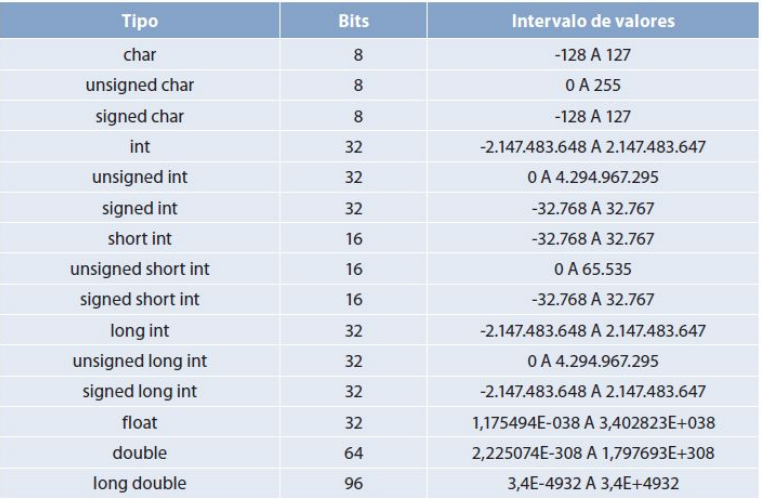
\includegraphics[width=8cm,height=7cm,keepaspectratio=false]{imagens/tipos.png}
	
	\end{center}
	
	\subsection{Input e output}
	Input e output é basicamente a entrada e a saída de dados. As vezes, podemos querer receber do usuário alguns valores, para fazer alguma coisa com eles e depois entregá-los com modificações. É basicamente isso. Um detalhe é que para o output, não necessariamente nós precisamos ter recebido algo.
	\subsubsection{Especificadores de formato}
	\subsubsection{Saída com printf()}
	Vamos começar com a saída de dados. Para exibir algo na tela. Fazemos:
	\begin{figure}[ht]
		\centering
		% ajusta a largura da imagem para ser quadrada (ex: 5cm x 5cm)
		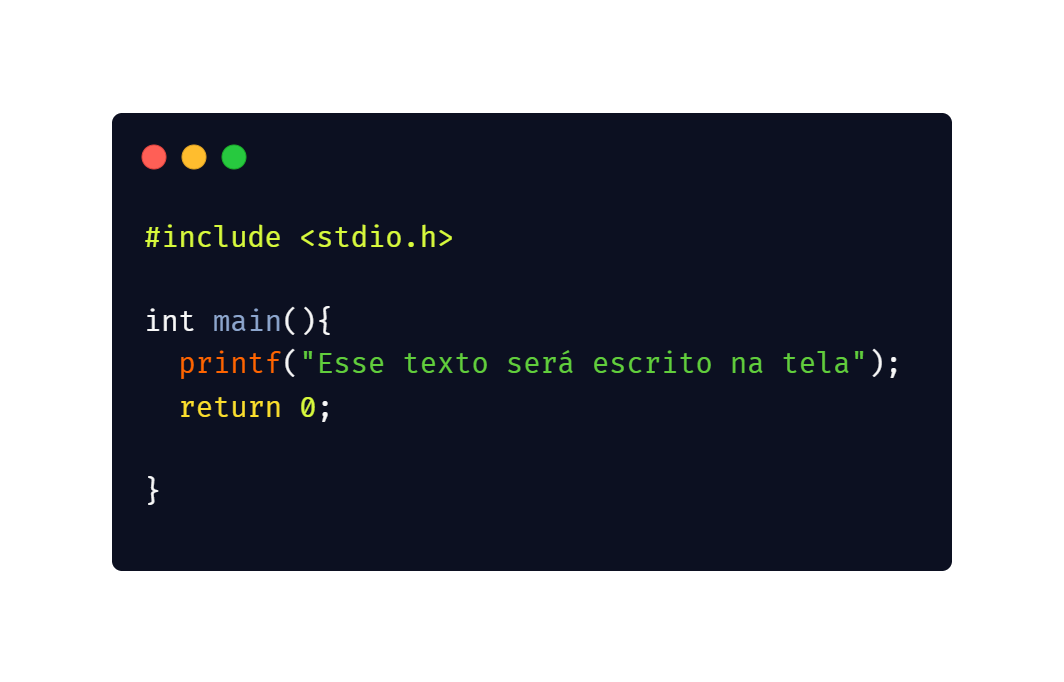
\includegraphics[width=6cm,height=3cm,keepaspectratio=false]{imagens/print.png}
		
	\end{figure}
	
	Ao fazer isso, em nosso terminal será exibido o texto que digitamos dentro do printf ("Esse texto será escrito na tela). Veja:
	
	\begin{center}
		
		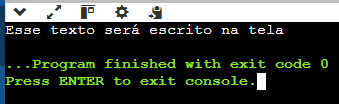
\includegraphics[width=7cm,height=2cm,keepaspectratio=false]{imagens/outputc.png}
	\end{center}
	
	\subsubsection{Uso do escape no printf()}
	Um detalhe é que algo que podemos utiliza no printf é caracter de escape . Esse caracter é utilizado sempre ao final do que que queremos escrever na saída e ele serve para quebrar a linha após a saída. Veja:
	
	\begin{figure}[ht]
		\centering
		% ajusta a largura da imagem para ser quadrada (ex: 5cm x 5cm)
		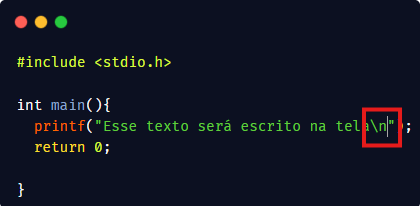
\includegraphics[width=6cm,height=3cm,keepaspectratio=false]{imagens/escape.png}
		
	\end{figure}
	
	
	Se fizermos vários printf, por exemplo, e não usarmos o caracter de escape em nenhum deles, o que escrevemos nos prints, ficará tudo junto. Veja:
	
	\begin{figure}[ht]
		\centering
		% ajusta a largura da imagem para ser quadrada (ex: 5cm x 5cm)
		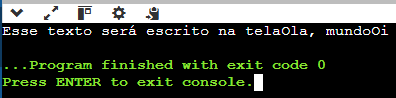
\includegraphics[width=6cm,height=3cm,keepaspectratio=false]{imagens/noescape.png}
	\end{figure}
	
	\subsubsection{Exibindo valores de variaveis no output}
	Se quisermos que em nosso output seja usada alguma variavel, temos que utilizar o seguinte formato:
	
	\begin{figure}[ht]
		\centering
		% ajusta a largura da imagem para ser quadrada (ex: 5cm x 5cm)
		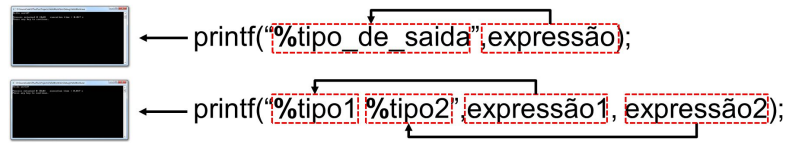
\includegraphics[width=9cm,height=2cm,keepaspectratio=false]{imagens/tipo_saida.png}
	\end{figure}
	
	Isso acima significa que se quisermos passar no output uma variavel que tenha o tipo int, nós teríamos que passar o tipo de saida  dentro das aspas duplas e depois separar por virgula passando a nossa variavel. Mas você deve estar se perguntando: Como assim tipos de saida? Veja abaixo os tipos de saida que usaremos no output (printf):
	
	\begin{center}

		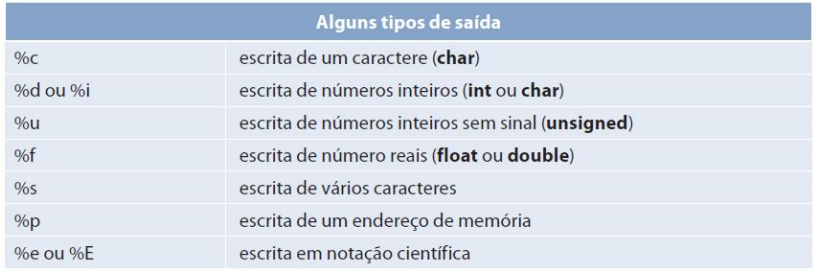
\includegraphics[width=8cm,height=3cm,keepaspectratio=false]{imagens/comando_saida.png}
	\end{center}
	
	Ou seja, seguindo o exemplo da variavel de tipo int que tinhamos dado, se quiséssemos exibi-la no output (printf), faríamos:
	
	\begin{LARGE}
		\begin{center}
			printf("porcentagemd", variavel);
		\end{center}
	\end{LARGE}
	
	\subsubsection{Entrada com scanf()}
	Agora, falando sobre entrada de dados, o comando que utilizamos para passar dados para o nosso programa é o scanf(). Esse comando permite realizar a leitura de dados da entrada padrão (teclado). Sua estrutura é a seguinte:
	
	\begin{center}
		
		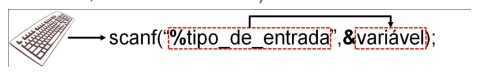
\includegraphics[width=7cm,height=2cm,keepaspectratio=false]{imagens/inputar.png}
	\end{center}
	
	Sendo que, os tipos de entrada são praticamente os mesmos que vimos nos tipos de saida. Veja:
	
	\begin{center}
		
		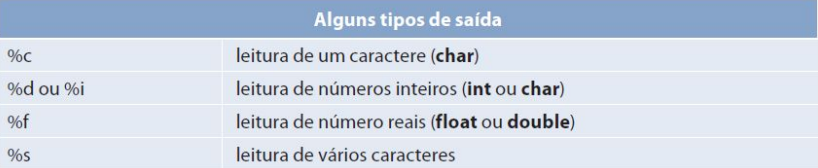
\includegraphics[width=7cm,height=2cm,keepaspectratio=false]{imagens/tipos_entrada.png}
	\end{center}
	
	Podemos ainda realizar a leitura de mais de um valor (assim como podemos fazer o output de mais de um valor). É bem parecido com o output também. Veja:
	
	
	\begin{center}
		
		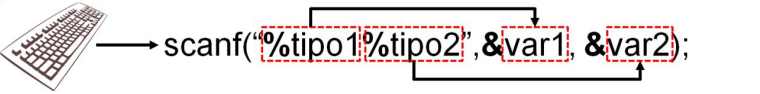
\includegraphics[width=7cm,height=2cm,keepaspectratio=false]{imagens/inputar_varios.png}
	\end{center}
	
	
	\subsection{Contantes}
	Assim como variaveis, constantes também armazenam um valor na memória do computador. A principal diferença para as variaveis é que esse valor não será alterado. Outra coisa é que para as constantes é obrigatoria a atribuição de valor, diferente das variaveis que podemos simplesmente declará-las sem dar um valor
	\subsubsection{Declaração de constantes}
	Para declarar uma constante existem duas formas. Na primeira, devemos  utilizar define nome-costante <valor> no começo do programa. Uma detalhe é que neste caso, não usaremos ponto e virgula no final. Veja:
	
	\begin{center}
		
		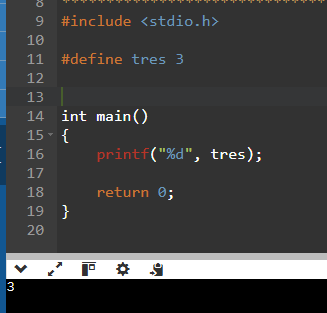
\includegraphics[width=5cm,height=4cm,keepaspectratio=false]{imagens/define.png}
	\end{center}
	
	Outra forma é fazer: const <tipo> nome = valor;. Como você pôde ver, nesse caso, temos que usar o ponto e vírgula. Veja:
	
	\begin{center}
	
	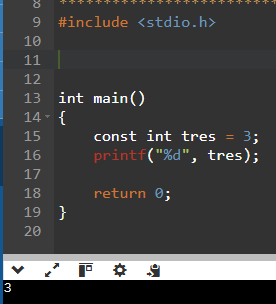
\includegraphics[width=5cm,height=4cm,keepaspectratio=false]{imagens/const.png}
	\end{center}	
	
	\subsubsection{Curiosidade sobre constantes}
	Já chegamos a falar sobre caracteres de escape (no caso, falamos apenas do barran). Os caracteres de escape são constantes pre-definidas. Veja cada um deles:
	
	\begin{center}
		
		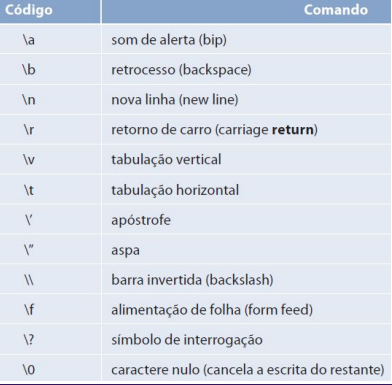
\includegraphics[width=7cm,height=6cm,keepaspectratio=false]{imagens/outros_escape.png}
		
	\end{center}
	
	
	\subsection{Operadores}
	Os operadores são usados para desenvolver diferentes tipos de operações. Com eles podemos fazer operações matematicas, comparativas, logicas e etc. Veremos acerca de cada um dos operadores a seguir
	\subsubsection{Operadores aritméticos}
	Os operadores aritméticos são aqueles que operam sobre numeros e/ou sobre expressões que tem como resultado valores numéricos. Veja os operadores:
	
	\begin{center}
		
		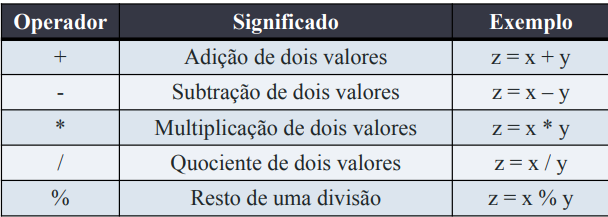
\includegraphics[width=6cm,height=3cm,keepaspectratio=false]{imagens/operadoresa.png}
		
	\end{center}
	
	Um detalhe é que as operações seguem a mesma ordem da matemática. A prioridade são as operações de multiplicação e divisão em detrimento das de soma e subtração.
	
	Outro detalhe é que na divisão, se o numerador e denominador forem inteiros, o compilador retornará apenas a parte inteira da divisão
	
	\subsubsection{Operadores relacionais}
	São aqueles que verificam a magnitude (maior/menor) e/ou igualdades entre dois valores e/ou expressões. Esses operadores retornam verdadeiro (1) ou falso (0) (ou seja, um valor booleano). Veja cada um deles:
	
	\begin{center}
		
		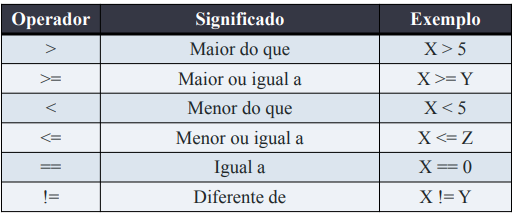
\includegraphics[width=6cm,height=3cm,keepaspectratio=false]{imagens/relacionais.png}
		
	\end{center}
	
	
	\subsubsection{Operadores lógicos}
	
	Os operadores lógicos nos permitem representar situações lógicas unindo duas mais expressões relacionais simples em uma composta e nos retornam verdadeiro (1) ou falso (0). Veja cada um deles:
	
	\begin{center}
		
		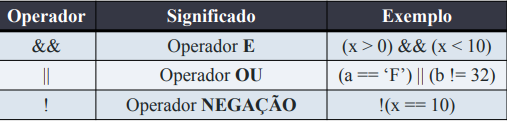
\includegraphics[width=7cm,height=2cm,keepaspectratio=false]{imagens/logicos.png}
		
	\end{center}
	
	\subsubsection{Operadores de atribuição simplificada}
	Muitas vezes em nosso código nós temos que atribuir valores a nossa variavel. Uma forma de fazer isso de maneira mais fácil é utilizando os operadores de atribuição simplificada. Com eles, podemos adicionar valores a nossa variavel de forma muito mais simples. Veja cada um deles:
	
	\begin{center}
		
		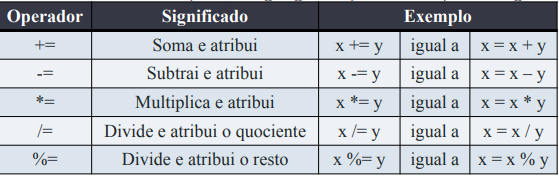
\includegraphics[width=7cm,height=2cm,keepaspectratio=false]{imagens/operadoresatribuicaosimp.png}
		
	\end{center}
	
	
	\subsubsection{Operadores de pré e pós incremento}
	Esses operadores podem ser utilizados sempre que for necessário somar uma unidade (incremento) ou subtrair uma unidade (decremento) a determinado valor. Veja cada um deles:
	
	\begin{center}
		
		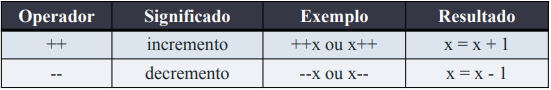
\includegraphics[width=8cm,height=2cm,keepaspectratio=false]{imagens/pospre.png}
		
	\end{center}
	
	Um detalhe é que como você pode ver na imagem acima, podemos utilizar o operador antes de depois da variavel, mas qual a diferença? Veja abaixo:
	
	\begin{center}
		
		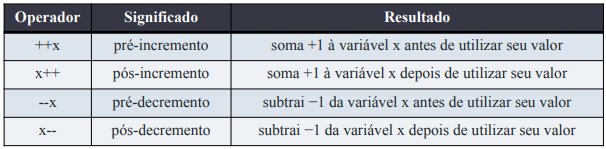
\includegraphics[width=8cm,height=3cm,keepaspectratio=false]{imagens/expliqprepos.png}
		
	\end{center}
	
	\subsection{Coerção de tipos}
	Lembra quando falamos anteriormente que se dividirmos um numero inteiro por outro inteiro seu resultado sempre será inteiro, desconsiderando assim a parte decimal? Podemos contornar isso utilizando o casting. O casting é aplicado sobre uma expressão aritmética e força o resultado da expressão a ser de um tipo especificado. Veja as diferentes formas de utilizar o casting:
	
		
	
	\subsubsection{Type casting explicito}
	Nós faremos a conversão de tipo no resultado da expressão:
	
	\begin{center}
		
		\begin{lstlisting}{caption=casting explicito em C, language=C, label=clanguage}
	int a = 5, b = 2;
	float resultado = (float)a / b;
	printf("%f\n", resultado);  // saida: 2.500000
			
			
		\end{lstlisting}
	\end{center}
	
	\subsubsection{Type casting nos operandos}
	Faremos o casting nos dois operandos da operação para obter o resultado no tipo que queremos
	
	\begin{center}
		
		\begin{lstlisting}{caption=casting explicito em C, language=C, label=clanguage}
	double resultado = (double)a / (double)b;
	printf("%lf\n", resultado); // saida: 2.500000

			
			
		\end{lstlisting}
	\end{center}
	
	\subsection{Condicionais}
	Certo. Agora falaremos sobre condicionais. Condicional é basicamente uma mudança de fluxo em nosso código. Caso uma determinada expressão atenda determinada condição, nosso código seguirá por um fluxo e caso contrário, seguirá para outro fluxo. Existem diferentes maneiras de se utilizar as condicionais em nosso código. Veremos cada uma delas abaixo.
	\subsubsection{If-else}
	A estrutura do if-else é feita da seguinte forma em nosso código:
	
	\begin{center}
		
		\begin{lstlisting}{caption=casting explicito em C, language=C, label=clanguage}
	if(condicao){
		sequencia de comandos 1;
	}
	else{
		sequencia de comandos 2;
	}
			
		\end{lstlisting}
	\end{center}
	
	
	O que acontece acima é que se a condição for satisfeita, ou seja, for verdadeira (tiver valor 1), nosso programa entrará nesse fluxo e executará o código dentro da condição. Caso contrário, ou seja, caso a condição não for satisfeita (for falsa (ter valor 0)), entraremos no fluxo do else.
	
	Um detalhe é que alem do if e do else, podemos ter ainda o else if, onde caso a condição do if não for satisfeita, haverá a condiçao do else if a ser satisfeita e aí se ela não satisfeita também, iremos para o else. Veja:
	
	\begin{center}
		
		\begin{lstlisting}{caption=casting explicito em C, language=C, label=clanguage}
	if(condicao){
		sequencia de comandos 1;
	}
	else if(condicao){
		sequencia de comandos 2;
	}
	else{
		sequencia de comandos 3;
	}
			
		\end{lstlisting}
	\end{center}
	
	\subsubsection{Swicth-case}
	O switch-case é outra estrutura de controle de fluxo de código. Sua estrutura é a seguinte:
	
	\begin{center}
		
		\begin{lstlisting}{caption=casting explicito em C, language=C, label=clanguage}
	switch(expressao){
		case valor 1:
			sequencia de comandos 1;
			break;
		
		case valor k:
			sequencia de comandos k;
			break;
		...
		default:
			sequencia de comandos padrao;
			break;
		
			
		\end{lstlisting}
	\end{center}
	
	O o switch, como podemos ver acima é próprio para testar uma variavel em relação a diversos valores pré-estabelecidos. Além disso, como podemos ver acima o default irá desempenhar o valor que o else desempenha na estrutura if-else
	\subsection{Loops}
	Agora falando sobre loops, o nome já entrega. Os loops serão responsáveis por repetir um bloco de código a partir de uma condição. Enquanto a condição for verdadeira, o bloco de código permanecerá se repetindo. Existem diferentes tipos de loops. Vamos a cada um deles.
	
	\subsubsection{While}
	\subsubsection{Do-While}
	\subsubsection{For}
	\subsection{Arrays}
	Quando vimos sobre variaveis, estudamos que elas podem armazenar um valor. Sempre que tentamos armazenar um novo valor dentro da variavel o antigo valor é sobrescrito (e portanto, perdido). Agora, pense: E se quisessemos armazenar mais de um valor em uma variavel? Para isso, usamos os arrays, que é basicamente uma sequencia de elementos do mesmo tipo, onde cada elemento é identificado por um indice. Ou seja, quando criamos um array, nós alocamos um espaço na memória (onde, quanto maior o tamanho do array, que é a quantidade de elementos que ele pode armazenar, maior o espaço de memoria alocado) e podemos armazenar dentro dele varios valores do mesmo tipo (os valores podem ser acessados por meio do indice do elemento dentro do array, que é basicamente a posição do elemento lá dentro). Um exemplo que pode fazer você entender melhor é: suponhamos que queiramos armazenar em um local a nota de 5 alunos. Para isso, poderiamos usar um array.
	\subsubsection{Declaração de arrays}
	Para declarar um array, nós fazemos da seguinte forma:
	
	\begin{LARGE}
		\begin{center}
			<tipo-array> nome-array[tamanho];
		\end{center}
	\end{LARGE}
	
	Ou seja, primeiro nós precisamos declarar o tipo do array, que será o tipo dos valores que aquele array irá armazenar, depois passamos o nome do array e depois passamos o tamanho do array, ou seja, a quantidade de elementos que ele poderá armazenar.
	
	
	
	\subsubsection{Inserindo e acessando valores dentro de arrays}
	Com o array declarado, caso quisermos inserir algum valor no array, basta fazer: 
	
	\begin{LARGE}
		\begin{center}
			nome-array[indice] = valor;
		\end{center}
	\end{LARGE}
	Lembrando que o indice é a posição do elemento dentro do array. Se tivessemos um array de tamanho 10 e quisessemos inserir um valor no sexto elemento, faríamos: nome-array[5] = valor; (uma vez que os indices começariam do 0 e iriam até o 9).
	
	Para acessar valores de um array, basta fazer:
	
	
	\begin{LARGE}
		\begin{center}
			nome-array[indice];
		\end{center}
	\end{LARGE}
	
	
	\subsubsection{Observações}
	Em C e C++, se tivermos um array que pode armazenar 10 elementos e tentarmos armazenar 11 elementos, o elemento que sobrar irá ser armazenado em um espaço da memória que não pertence ao array, o que causa comportamento indefinido (pode sobrescrever dados, travar o programa e entre outros)
	
	Outro detalhe é que se tivermos um array de 10 elementos (ou seja, teremos 10 indices, do 0 ao 9) e tentarmos acessar o indice 10 (11º elemento) o que acontecerá (em C e C++) é que iremos acessar um elemento da memória que não pertence oficialmente ao array, o que pode retornar "Lixos de memória".
	
	
	\subsection{Struct - Criação de tipos}
	Agora, falaremos sobre structs, estamos falando de uma composição de variaveis de outros tipos que formam um "novo tipo de dado". Assim como temos o tipo inteiro, float e etc, podemos "criar" um outro tipo que será um agrupamento de dados.
	\subsubsection{Declaração}
	
	\subsubsection{Inserindo valores e acessando valores}
	
	\subsection{Comando typedef}
	O comando typedef nos permite "dar um alias" para os tipos de dados existentes na linguagem C. Se temos, por exemplo, o tipo float, mas queremos que ele se chame flutuante, poderíamos fazer isso. 
	\subsubsection{Como usar}
	Para usar, basta fazer o seguinte:
	
	\begin{LARGE}
		\begin{center}
			typedef <tipo-de-dado> <alias>;
		\end{center}
	\end{LARGE}
	
	O comando acima "da um alias" a um tipo de dado existente. Um detalhe é que o comando acima deve estar no topo do programa, juntamente com a inclusão das bibliotecas.
	
	\subsubsection{Exemplo}
	
	\chapter{Acerca de ponteiros}
	\section{O porquê de estudar esse topico}
	Agora, iniciaremos um tópico mais avançado, que são os ponteiros. É muito importante entendermos sobre esse conceito porque várias das estruturas de dados que aprenderemos nesta disciplina dependem deles (listas, pilhas, filas, árvores e grafos), então sem entender isso, não iremos para frente
	\section{O que são e como usá-los}
	\subsection{O que é}
	Conceitualmente, um ponteiro é uma variavel que armazena o endereço de memoria de outra variavel. Ou seja, diferentemente das variaveis comuns, um ponteiro não irá armazenar um valor como um caracter, por exemplo, mas sim, um endereço de memória.	
	\subsection{Declaração de ponteiros}
	Para criar um ponteiro, a estrutura lembra bastante a forma como nós criamos as variaveis, mas com pequenas mudanças. Veja como declaramos um ponteiro:
	
	\begin{LARGE}
		\begin{center}
			<tipo de dado> *nome ponteiro;
		\end{center}
	\end{LARGE}
	
	Perceba que para declarar um ponteiro, assim como nas variaveis, nós temos que usar um tipo de dado. Isso acontece porque nós estamos indicando para o ponteiro que estamos criando o tipo de dado do lugar da memória que ele vai apontar. Isso é importante porque não é muito aconcelhavel você ter um ponteiro inteiro e apontar para um char, por exemplo.
	
	Um detalhe é que podemos criar o nosso ponteiro apontando ele para NULL, para que ele não aponte para nenhum lugar (para que consigamos administrar para onde ele aponta depois). Fazendo isso, a declaração ficaria:
	
	\begin{LARGE}
		\begin{center}
			<tipo de dado> *nome ponteiro = NULL;
		\end{center}
	\end{LARGE}
	
	Se não declararmos da maneira acima e utilizarmos a primeira versão de declaração (<tipo de dado> *nome ponteiro;), o que acontece é que nosso ponteiro irá apontar para um endereço de memória aletório.
	
	Um outro detalhe bem interessante é que podemos fazer com que nosso ponteiro aponte para o endereço de memória de uma variavel já existente. Veja:
	
	\begin{LARGE}
		\begin{center}
			<tipo de dado> *nome ponteiro = \&a;
		\end{center}
	\end{LARGE}
	
	
	Ou seja, o endereço de memória que nosso ponteiro irá apontar, será o endereço da variavel a (esse  significa que estamos nos referindo ao endereço de memoria da variavel a. Desta forma, o ponteiro b apontará para o endereço de memoria de a).
	
	\subsection{Detalhe após a declaração}
	
	Quando declaramos um ponteiro(exemplo: int *a), algo importante de se dizer é que se utilizarmos *a em qualquer outro trecho do nosso código, nós não vamos estar usando o ponteiro em si, mas sim o valor que está no endereço apontado pelo ponteiro a. Veja um exemplo:
	
	\begin{center}
		
		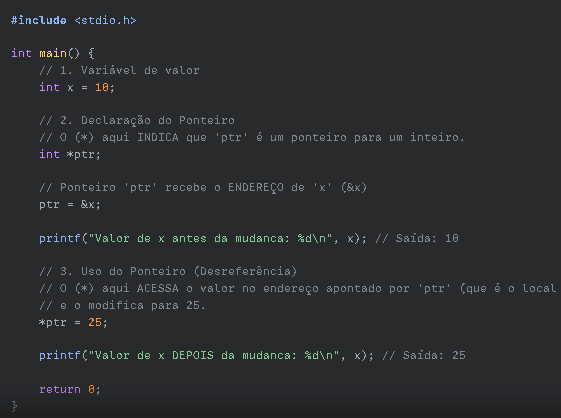
\includegraphics[width=10cm,height=8cm,keepaspectratio=false]{imagens/pointer.png}
		
	\end{center}
	
	
	\subsection{Exemplo de uso}
	Veja abaixo um exemplo de uso de ponteiros:
	
	\begin{figure}[ht]
		\centering
		% ajusta a largura da imagem para ser quadrada (ex: 5cm x 5cm)
		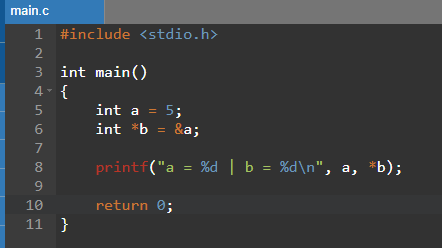
\includegraphics[width=7cm,height=4cm,keepaspectratio=false]{imagens/ponteiro.png}
		
	\end{figure}
	
	Acima, o que acontece é que:
	
	\begin{itemize}
		\item int a = 5; -> Declara uma variável do tipo inteiro chamada a e a inicializa com o valor 5. A variável a armazena o valor 5 em um local específico da memória
		\item int *b = \&a; -> O *b declara uma variável chamada b como um ponteiro para um inteiro (int *). O operador endereço de (\&) é usado para obter o endereço de memória onde a variável a está armazenada. O ponteiro b é, portanto, inicializado para armazenar o endereço de memória de a. O valor de b não é 5, mas sim o endereço onde o 5 está guardado.
		\item parte do printf -> O primeiro \%d exibe o valor da variável a, que é 5. O segundo \%d exibe o valor armazenado no endereço apontado por b. O operador desreferência ou conteúdo de (*) é usado em frente ao ponteiro b para acessar o valor guardado naquele endereço—ou seja, o valor de a, que também é 5.
	\end{itemize}
	
	\chapter{Falando de funções}
	
	\section{O que é}
	Funções são blocos de código que podem ser nomeados e chamados dentro de um programa. Elas facilitam a estruturação e reutilização do código, pois:
	
	\begin{itemize}
		\item Estruturação: programas grandes e complexos são construídos bloco a bloco.
		\item Reutilização: o uso de funções evita a cópia desnecessária de trechos de código que realizam a mesma tarefa, diminuindo assim o tamanho do programa e a ocorrência de erros
	\end{itemize}
	
	\section{Estrutura}
	A forma geral de uma função é:
	
	\begin{center}
		
		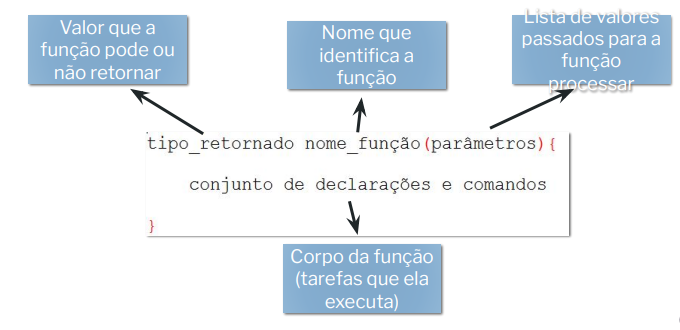
\includegraphics[width=12cm,height=4cm,keepaspectratio=false]{imagens/func.png}
		
	\end{center}
	
	As funções devem ser declaradas ANTES de serem utilizadas, ou seja, antes da cláusula main
	
	\subsection{Corpo}
	
	O corpo é a alma da função e é composto pelos comandos que a função deve executar. Ele processa os parametros (se houver), realiza tarefas e gera saídas (se necessário)
	
	Um detalhe é que nós evitamos operações de leitura e escrita dentro de uma função. Essas operações devem ser feitas em quem chamou a função (o main()), por exemplo.
	
	\subsection{Parametros}
	
	A declaração de parametros é uma lista de variaveis juntamente com seus tipos: tipo1 nome1, tipo2 nome2...
	
	\begin{center}
		
		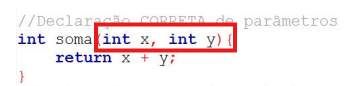
\includegraphics[width=12cm,height=4cm,keepaspectratio=false]{imagens/parametros.png}
		
	\end{center}
	
	É por meio dos parâmetros que uma função recebe informação do programa principal (isto é, de quem a chamou)
	
	Um detalhe é que podemos criar funções que não recebem nenhum parametro. Isso pode ser deito de duas formas:
	
	\begin{center}
		
		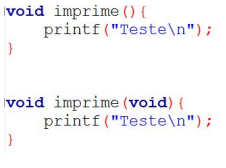
\includegraphics[width=6cm,height=3cm,keepaspectratio=false]{imagens/parametros2.png}
		
	\end{center}
	
	
	
	\subsection{Retorno}
	
	As funções podem ou não retornar algum valor. Se ela retornar, alguém deverá receber este valor (os valores retornados de funções devem ser armazenados em uma varíavel)
	
	O retorno da função é dado pelo comando:
	
	\begin{center}
		\begin{LARGE}
			return valor ou exepressao;
		\end{LARGE}
	\end{center}
	
	É importante lembrar que o valor de retorno fornecido tem que ser compatível com o tipo de retorno declarado para a função

	Uma função que retorna nada é definida colocando-se o tipo void como valor retornado
	
	\begin{center}
		
		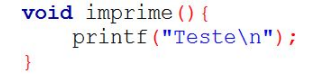
\includegraphics[width=6cm,height=3cm,keepaspectratio=false]{imagens/retorno.png}
		
	\end{center}
	
	Uma função pode ter mais de uma declaração return. Quando um comando return é executado, a função termina imediatamente.

	\subsection{Escopo}
	
	Assim como em nosso programa principal, as funções também estão sujeitas ao escopo das variaveis. Escopo é o conjunto de regras que determinam o uso e a validade de variaveis nas diversas partes do programa:
	
	\begin{itemize}
		\item Variaveis Locais: São aquelas que só tem validade no bloco onde são declaradas. Exemplo: variaveis declaradas dentro da função
		\item Variaveis Globais: São declaradas fora de todas as funções do programa. Elas são conhecidas e podem ser alteradas por todas as funções do programa	
	\end{itemize}
	
	
	\section{Passagem de parâmetros}
	
	
	\subsection{Passagem por valor}
	Na linguagem C, os parametros de uma função são, por padrão, passados por valor, ou seja, uma cópia do valor do parametro é feita e passada para a função. Mesmo que esse valor mude dentro da função, nada acontece com o valor de fora da função
	\subsection{Passagem por referência}
	Quando se quer que o valor da variavel mude dentro da função, usa-se passagem de parâmetros por referência.
	
	Nesse tipo de chamada, não se passa para a função o valor da varíavel, mas sim sua referencia (seu endereço de memoria), assim qualquer alteração que a variavel sofra dentro da função será refletida fora da função. Um exemplo disso é a função scanf(), onde sempre que desejamos ler um valor, passamos essa função o endereço de memoria da variavel que queremos armazenar o valor recolhido, ou seja, a variavel que usamos terá seu valor modificado dentro da função scanf(), e seu valor pode ser acessado no programa principal. Veja um outro exemplo:
	
	Como podemos ver acima, para passar um parametro por referencia, coloca-se um asterisco na frente do nome do parametro na declaração da função. A partir disso, ao chamar a função, será necessario passar o operador \&, assim como é feito com scanf()
	
	\begin{center}
		
		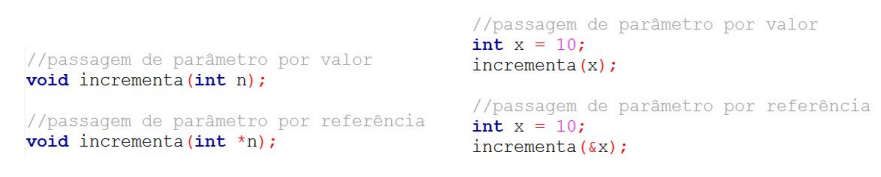
\includegraphics[width=13cm,height=3cm,keepaspectratio=false]{imagens/referencia.png}
		
	\end{center}
	
	\subsection{Arrays como parametro}
	
	Para utilizar arrays como parametros de funções alguns cuidados simples são necessários
	
	\begin{itemize}
		\item Arrays são sempre passados por referência para uma função. A passagem de arrays por referencia evita a cópia desnecessária de grandes quantidades de dados para outras áreas de memória durante a chamada da função, o que afetaria o desempenho do programa
		\item É necessário declarar um segundo parametro (em geral uma variavel inteira) para passar para a função o tamanho do array separadamente 
		\item Quando passamos um array por parametro , independente do seu tipo, o que é de fato passado é o endereço do primeiro elemento do array
	\end{itemize}
	
	Na passagem de um array como parametro de uma função podemos declarar a função de diferente maneiras, todas equivalentes:
	
	\begin{center}
		
		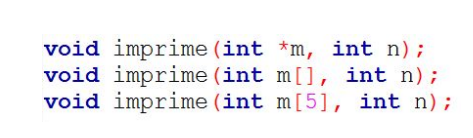
\includegraphics[width=8cm,height=3cm,keepaspectratio=false]{imagens/funcarray.png}
		
	\end{center}
	
	
	
	\subsection{Struct como parametro}
	
	\section{Recursão}
	
	\chapter{Introdução aos algoritmos}
	\section{Algoritmos de busca}
	Quando temos um conjunto de dados, podemos querer procurar por um elemento. Exemplo: Temos um array de números inteiros, pode ser que queiramos buscar algum valor dentro desse array.
	
	Existem varios tipos de busca e a utilização dos tipos dependerá de como são os dados (se eles estão estruturados, ordenados e se existem valores duplicados). Com isso em mente, veremos cada um desses tipos de busca
	\subsection{Busca linear - Não ordenada}
	
	\subsubsection{Como funciona?}
	
	Esse é o algoritmo de busca mais simples que existe. O que ele faz é percorrer o array que contém os dados desde sua primeira posição até a última comparando cada valor dele com o valor buscado. Se os valores forem iguais, a busca termina e caso contrário, continua até o fim do array.
	
	
	\begin{center}
		
		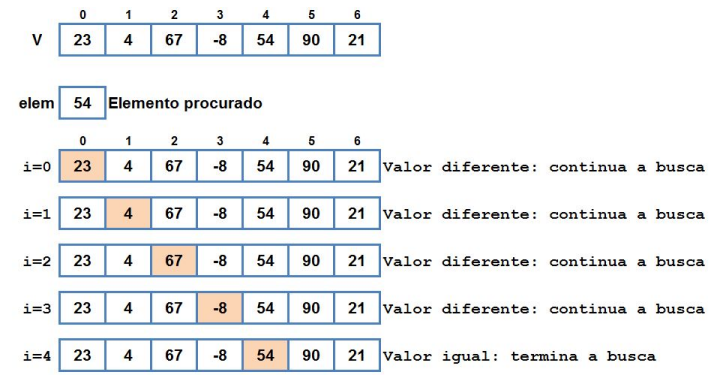
\includegraphics[width=10cm,height=4cm,keepaspectratio=false]{imagens/blinearfuncionamento.png}
		
	\end{center}
	
	Apesar de ser intuitivo, o motivo pelo qual ele tem que percorrer o array inteiro é o fato dele não estar ordenado. No nosso exemplo, suponhamos que o array estivesse ordenado, mas que o número 54 que está sendo buscado não existisse. Ao fazer nossa busca, quando chegarmos no número 67, ele iria parar a busca, pois o valor procurado não poderia estar depois de 67 (o array está ordenado).
	\subsubsection{Complexidade}
	
	A complexidade do algoritmo de busca linear não ordenada pode ser analisada conforme os seguintes casos:
	
	\begin{itemize}
		\item Melhor caso: O(1). Acontece quando o elemento buscado é o primeiro do array.
		\item Pior caso: O(N). Acontece quando o elemento é o último do array ou não existe.
		\item Caso médio: O(N/2). 
	\end{itemize}
	
	\subsubsection{Implementação}
	
	\begin{center}
		
		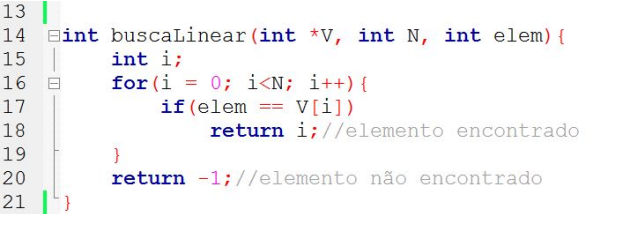
\includegraphics[width=8cm,height=3cm,keepaspectratio=false]{imagens/blinear.png}
		
	\end{center}
	
	\subsection{Busca linear - Ordenada}
	\subsubsection{Como funciona?}
	A busca sequencial ordenada funcionará da mesma forma que a busca sequencial não ordenada. A diferença é que, com o array ordenado, caso o valor do array seja maior que o valor buscado, ele parará a busca.
	
	\begin{center}
	
	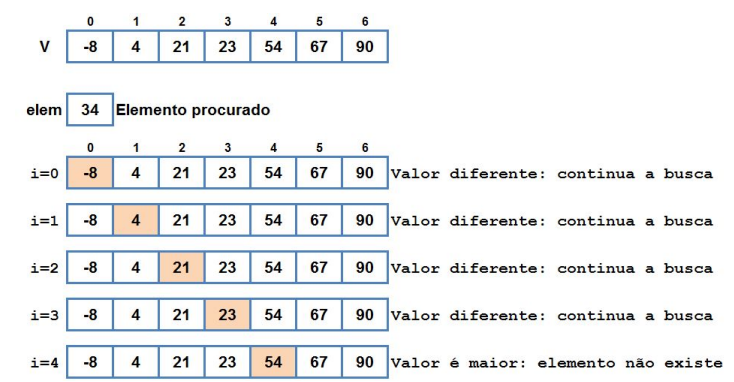
\includegraphics[width=10cm,height=4cm,keepaspectratio=false]{imagens/blinearordenada.png}
	
	\end{center}
	
	\subsubsection{Complexidade}
	
	A complexidade do algoritmo de busca linear ordenada pode ser analisada conforme os seguintes casos:
	
	\begin{itemize}
		\item Pior caso: O(n). Acontece quando o valor é o maior valor do array, ou seja, está na última posição do array
	\end{itemize}
	
	\subsubsection{Implementação}
	
	\begin{center}
		
		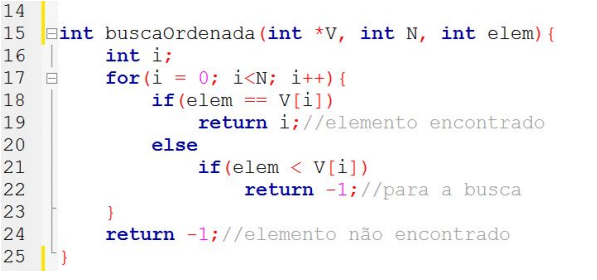
\includegraphics[width=10cm,height=4cm,keepaspectratio=false]{imagens/blinearordenadafuncionamento.png}
		
	\end{center}
	
	\subsection{Busca Binária}
	
	\subsubsection{Como funciona?}
	
	Esse algoritmo é uma das formas mais "especializadas" de se realizar uma busca em um array. Para utilizá-lo o array DEVE estar ordenado. O que ele faz é calcular o meio do array e utilizar o valor desse meio para comparar com o valor buscado. Se o valor buscado for menor que o valor do meio, ele descarta a segunda metade do array e fica com apenas a primeira metade com os valores menos. Caso o valor buscado for maior, ele fará o contrário
	
	\begin{center}
		
		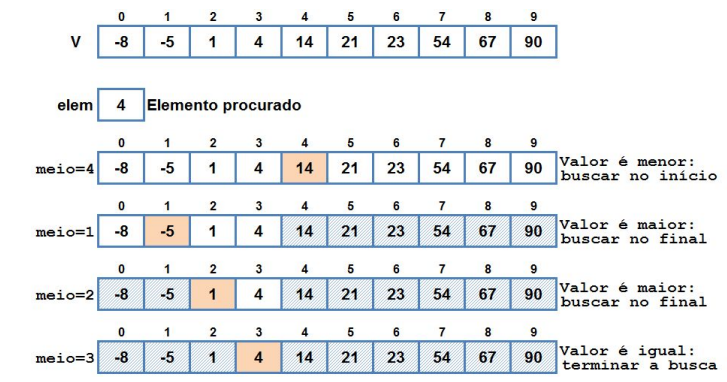
\includegraphics[width=10cm,height=4cm,keepaspectratio=false]{imagens/bbinaria.png}
		
	\end{center}
	
	A parte em azul na imagem acima representa a parte do array que foi descartada por conta da condição
	
	
	Um detalhe é que ao realizar a comparação entre o valor buscado e o valor do meio do array, ele vai verificar se o valor buscado é igual ao valor do meio do array e, caso for, ele já encerra a busca ali mesmo.
	
	\subsubsection{Complexidade}
	
	A complexidade do algoritmo de busca linear ordenada pode ser analisada conforme os seguintes casos:
	
	\begin{itemize}
		\item Melhor caso: O(1). O elemento está exatamente no meio do array
		\item Caso médio: O(log2 N). 
		\item Pior caso: O(log2 N). O elemento não existe
	\end{itemize}
	
	\subsubsection{Implementação}
	
	Abaixo, a sua implementação no código:
	
	\begin{center}
		
		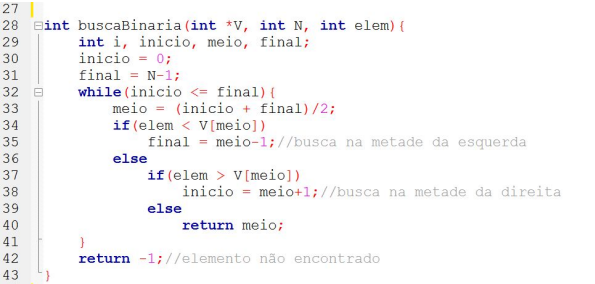
\includegraphics[width=10cm,height=4cm,keepaspectratio=false]{imagens/bbinariafunc.png}
		
	\end{center}
	
	\subsection{Busca em array de struct}
	\subsubsection{Como funciona?}
	
	Aqui, estamos lidando com algo mais complexo. Quando queremos buscar algo em um array de struct, nós usaremos uma das chaves da struct para realizar a busca, como usar a matricula para buscar de uma struct para realizar uma busca
	
	\begin{center}
		
		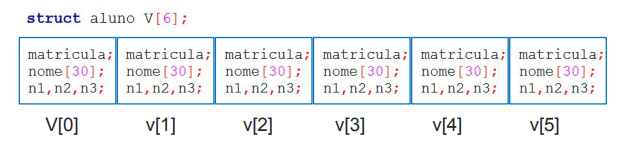
\includegraphics[width=10cm,height=4cm,keepaspectratio=false]{imagens/bstruct.png}
		
	\end{center}
	
	\subsubsection{Complexidade}
	
	Como estamos falando de uma busca linear, sua complexidade será a mesma
	
	\subsubsection{Implementação}
	
	\begin{center}
		
		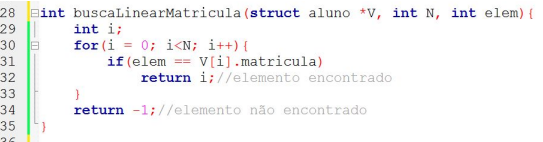
\includegraphics[width=8cm,height=3cm,keepaspectratio=false]{imagens/bstructimplement.png}
		
	\end{center}
	
	
	
	\section{Algoritmos de ordenação}
	Após uma base de dados estar construída pode ser necessário ordena-la. A ordenação dos dados PODE ser um passo preliminar para pesquisá-los (para utilizar o algoritmo de busca binária, por exemplo, precisamos que os dados estejam ordenados). Dada essa introdução, veremos alguns algoritmos de ordenação de dados.
	
	\subsection{Bubblesort}
	
	\subsubsection{Como funciona?}
	O algoritmo de ordenação bublesort  é o mais simples dos algoritmos de ordenção. O que ele faz é:
	
	\begin{enumerate}
		\item Comparação de dois números
		\item Se o da esquerda for maior, os elementos devem ser trocados
		\item Desloca-se uma posição à direita
	\end{enumerate}
	
	
	Exemplo: Estamos percorrendo um vetor e na posição da esquerda nós temos o número 10 e na posição da direita nós temos o número 8. Como 8 é menor que 10, iremos fazer a troca. No lugar do 10, teremos o 8 e no lugar do 8 teremos o 10. Feito isso, ele estará na posição onde está o valor 8, então ele irá se deslocar uma posição à direita (que é onde estará o valor 10).
	
	A medida que o algoritmo avança, os itens maiores "surgem como uma bolha" na extremidade superior do vetor (à direita do vetor). É por isso que o é o  algoritmo da bolha (bolha = bubble)
	
	Podemos observar essa algoritmo de forma visual a partir \href{ https://visualgo.net/en/sorting}{deste link}. Aqui vai um exemplo rápido com algumas imagens:


	\begin{figure}[h]
		\centering
		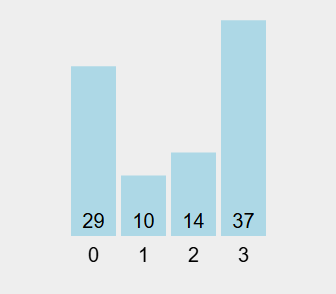
\includegraphics[width=0.45\textwidth]{imagens/bubble-sort1.png}
		\hfill
		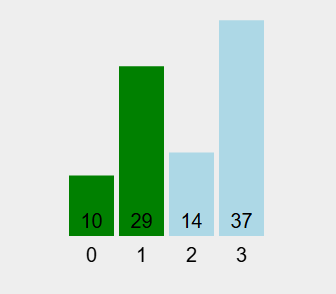
\includegraphics[width=0.45\textwidth]{imagens/bubble-sort2.png}

	\end{figure}
	
	\begin{figure}[h]
		\centering
		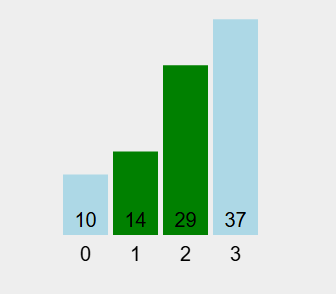
\includegraphics[width=0.45\textwidth]{imagens/bubble-sort3.png}
		\hfill
		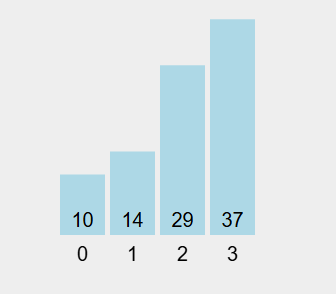
\includegraphics[width=0.45\textwidth]{imagens/bubble-sort4.png}
		
	\end{figure}

	Na primeira imagem, podemos ver o nosso vetor de forma desordenada, aí o que acontecerá com a aplicação do algoritmo de bubble sort é que pegaremos o número da esquerda (no caso 29) e iremos comparar com o segundo. Se o segundo número for menor, jogamos o maior para a direita (assim como podemos ver na segunda imagem, onde o número 29 foi para a direita e o 10, que era menor, foi para a esquerda). Após isso, faremos a comparação novamente entre o número da esquerda e o da direita. Agora, estamos comparando o 29 (esquerda) e o 14 (direita), então como o número da esquerda é maior (29), iremos joga-lo para a direita e o número que estava na direita virá para a esquerda, assim como podemos ver na terceira imagem. Por fim, vamos fazer a comparação novamente entre o número da esquerda e o da direita. Dessa vez o número da esquerda é menor que o da direita, então não haverá troca, aí passaremos para o próximo número (37) para realizar novas comparações, mas como o vetor acabou, então finalizamos por aqui.
	
	Portanto, o algoritmo vai percorrendo o vetor e fazendo as trocas, mas pode ser que ele tenha que percorrer o vetor mais de uma vez para fazer a ordenação (na maioria das vezes é o que acontece, apesar de termos dado sorte no exemplo que demos acima). Apesar disso, uma coisa que ele garante é que após a primeira rodada o maior elemento do array será movido para a última posição do array e isso faz com que, para um vetor com n elementos, o Bubble Sort precise de no máximo n-1 passagens. Isso acontece porque a cada passagem, o maior elemento restante é movido para sua posição final correta. Após a n-1ª passagem, os n-1 maiores elementos já estarão ordenados. Por consequência, o único elemento que sobrou, o menor de todos, já estará automaticamente na primeira posição, que é a sua posição correta. Sendo assim, não há necessidade de uma n-ésima passagem.
	
	
	\subsubsection{Complexidade}
	Com relação ao Big-O desse algoritmo, ele é um O($n^{2}$), ou seja, o tempo de execução dele é relativamente grande:
	
	\begin{center}
		
		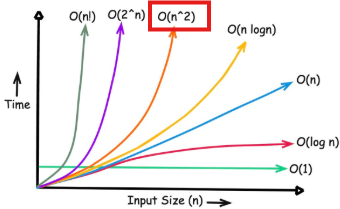
\includegraphics[width=7.5cm,height=4cm,keepaspectratio=false]{imagens/bubble_comple.png}
		
	\end{center}
	
	A razão que faz esse algoritmo ser um O($n^{2}$) é o fato de ter dois loops aninhados que o algoritmo usa para percorrer o vetor (veremos na implementação)
	
	
	\subsubsection{Implementação}
	
	\begin{center}
		
		\begin{lstlisting}{caption=casting explicito em C, language=C, label=clanguage}
#include <stdio.h>
	
//Funcao para trocar dois elementos de lugar
void trocar(int *a, int *b) {
	int temp = *a;
	*a = *b;
	*b = temp;
}
	
//Funcao que implementa o Bubble Sort
void bubbleSort(int vetor[], int n) {
	int i, j;
	int houveTroca;
		
	//O algoritmo precisa repetir varias vezes
	//ate que nao haja mais trocas
	for (i = 0; i < n - 1; i++) {
		houveTroca = 0; //no comeco da rodada, nao houve troca ainda
			
		//Percorre o vetor ate a penultima posicao comparando os vizinhos
		for (j = 0; j < n - i - 1; j++) {
			if (vetor[j] > vetor[j + 1]) {
				trocar(&vetor[j], &vetor[j + 1]);
				houveTroca = 1; // se houve troca, marcamos
			}
		}
			
		//Se nao houve troca, significa que o vetor ja esta ordenado
		if (houveTroca == 0) {
			break;
		}
	}
}
	
//Funcao para imprimir o vetor
void imprimirVetor(int vetor[], int n) {
	for (int i = 0; i < n; i++) {
		printf("%d ", vetor[i]);
	}
	printf("\n");
}
	
int main() {
	int vetor[] = {64, 34, 25, 12, 22, 11, 90};
	int n = sizeof(vetor) / sizeof(vetor[0]);
		
	printf("Vetor original: ");
	imprimirVetor(vetor, n);
		
	bubbleSort(vetor, n);
		
	printf("Vetor ordenado: ");
	imprimirVetor(vetor, n);
		
	return 0;
}
				
		\end{lstlisting}
	\end{center}
	
	Explicação da implementação:
	
	\begin{enumerate}
		\item void trocar(int *a, int*b)
		
		Essa é uma função auxiliar que serve para trocar os valores de duas variáveis inteiras.
		
		\begin{itemize}
			\item int *a e int *b: Os parâmetros são ponteiros para inteiros, e não as variáveis em si. Como sabemos, um ponteiro é uma variável que armazena o endereço de memória de outra variável. Usamos ponteiros aqui porque, para a função trocar realmente modificar os valores das variáveis que a chamaram, ela precisa de seus endereços de memória. Se passássemos apenas int a e int b, a função criaria cópias locais dos valores, e a troca não afetaria o vetor original.
			\item int temp = *a;: A variável temp (de "temporário") é usada para guardar o valor original do primeiro elemento. O asterisco (*) é o operador de desreferenciação; ele "desempacota" o ponteiro para acessar o valor que está no endereço de memória. Então, *a é o valor da variável que o ponteiro a está apontando.
			\item *a = *b;: O valor da segunda variável (*b) é atribuído à primeira (*a)
			\item *b = temp;: O valor original da primeira variável (*a), que estava guardado em temp, é atribuído à segunda (*b).
			
		\end{itemize}
		
		\item void bubbleSort(int vetor[], int n)
		
		Esta é a função principal que implementa o algoritmo de ordenação.
		
		\begin{itemize}
			\item for (i = 0; i < n - 1; i++): Este é o laço externo. Ele controla o número de "passagens" que o algoritmo fará pelo vetor. Em cada passagem, o maior elemento "flutua" para a sua posição correta no final do vetor. O n - 1 é usado porque, se temos n elementos, precisamos de no máximo n - 1 passagens para ordená-los.
			\item int houveTroca = 0;: Esta variável de controle é uma otimização do Bubble Sort. Ela é inicializada como 0 (falso) no início de cada passagem. Se o laço interno não realizar nenhuma troca, significa que o vetor já está ordenado, e podemos parar o algoritmo mais cedo.
			\item for (j = 0; j < n - i - 1; j++): Este é o laço interno. Ele é responsável por percorrer o vetor e comparar os pares de elementos vizinhos.
			\begin{itemize}
				\item n - i - 1: A cada passagem do laço externo (i), o maior elemento já está na sua posição correta no final. Portanto, não precisamos mais comparar os elementos que já estão no lugar certo. Por exemplo, na primeira passagem (i=0), o maior elemento vai para a última posição. Na segunda passagem (i=1), o segundo maior elemento vai para a penúltima posição, e assim por diante. Essa otimização evita comparações desnecessárias, melhorando a eficiência do algoritmo.
			\end{itemize}
			\item if (vetor[j] > vetor[j + 1]): Esta é a condição principal de comparação. Se o elemento atual (vetor[j]) for maior que o seu vizinho da direita (vetor[j + 1]), eles estão na ordem errada para uma ordenação crescente.
			\item trocar(\&vetor[j], \&vetor[j + 1]);: Com a condição sendo verdadeira, a função trocar é chamada. Note que usamos o operador \& (operador de endereço) para passar o endereço de memória dos elementos do vetor, pois a função trocar espera ponteiros.
			\item if (houveTroca == 0) { break; }: Esta é a otimização comentada antes. Se, depois de uma passagem completa do laço interno, a variável houveTroca ainda for 0, significa que o vetor está totalmente ordenado. Nesse caso, usamos o comando break para sair do laço externo, encerrando o algoritmo.
		\end{itemize}
		\item int main()
		
		Esta é a função principal do programa, onde a execução começa.
		
		\begin{itemize}
			\item int vetor[] = {64, 34, 25, 12, 22, 11, 90};: Declara e inicializa um vetor de inteiros com os valores a serem ordenados.
			
			\item int n = sizeof(vetor) / sizeof(vetor[0]);: Esta é uma forma padrão e portátil de calcular o número de elementos em um vetor em C.
			
			\begin{itemize}
				\item sizeof(vetor): Retorna o tamanho total do vetor em bytes.
				\item sizeof(vetor[0]): Retorna o tamanho de um único elemento do vetor em bytes (neste caso, o tamanho de um int).
				\item Ao dividir o tamanho total pelo tamanho de um elemento, obtemos o número exato de elementos no vetor, independentemente do tipo de dado ou da arquitetura do sistema. Isso é muito mais robusto do que simplesmente contar os elementos manualmente.
			\end{itemize}
			\item printf("Vetor original: "); e imprimirVetor(vetor, n);: Exibe o vetor antes da ordenação.
			\item bubbleSort(vetor, n);: Chama a função para ordenar o vetor.
			\item printf("Vetor ordenado: "); e imprimirVetor(vetor, n);: Exibe o vetor após a ordenação.
		\end{itemize}
	\end{enumerate}
	\subsection{Insertion sort}
	\subsubsection{Como funciona?}
	Também é um dos mais simples algoritmos de ordenação existentes. Ele possui um método de ordenação semelhante ao que usamos para
	ordenar as cartas de um baralho. O que ele faz é pegar uma carta de cada vez e a coloca em seu devido lugar, sempre deixando as cartas da mão em ordem.
	
	\begin{enumerate}
		\item 
	\end{enumerate}
	
	\subsubsection{Comlexidade}
	Os casos de complexidade
	
	\begin{itemize}
		\item Melhor caso: O(n). Ocorre quando a lista já está completamente ordenada.
		\item Caso médio: O(n²).
		\item Pior caso: O(n²).
	\end{itemize}
	\subsection{Selection sort}
	\subsubsection{Como funciona?}
	A idéia da ordenação por seleção é
	procurar o menor elemento do
	vetor (ou maior) e movimentá-lo
	para a primeira (última) posição do
	vetor. Repetir para os n elementos do
	vetor.
	\subsubsection{Complexidade}
	Sua complexidade:
	
	\begin{itemize}
		\item Melhor caso: O(n²)
		\item Caso médio: O(n²)
		\item Pior caso: O(n²)
	\end{itemize}
	
	\subsection{Merge sort}
	\subsubsection{Como funciona?}
	
	Também conhecido como ordenação por intercalação. É um Algoritmo recursivo que usa a idéia de dividir para conquistar para
	ordenar os dados (Parte do princípio de que é mais fácil ordenar um conjunto com poucos dados do que um com muitos). O algoritmo divide os dados em conjuntos cada vez menores para depois ordená-los e combina-los por meio de intercalação (merge)
	
	\begin{itemize}
		\item Divide, recursivamente, o conjunto de dados até que cada subconjunto possua 1 elemento
		\item Combina 2 subconjuntos de forma a obter 1 conjunto maior e ordenado
		\item Esse processo se repete até que exista apenas 1 conjunto
	\end{itemize}
	\subsubsection{Complexidade}
	\begin{itemize}
		\item Melhor caso: O(nlogn)
		\item Caso médio: O(nlogn)
		\item Pior caso: O(n log n)
	\end{itemize} 
	\subsection{Shell sort}
	\subsubsection{Como funciona?}
	\subsubsection{Complexidade}

	\subsection{Quicksort}
	\subsubsection{Como funciona?}
	
	É o algoritmo de ordenação interna mais rápido que se conhece para uma ampla variedade de situações. Provavelmente é o mais utilizado. Ideia básica: Dividir e Conquistar. Um elemento é escolhido como pivô. “Particionar”: os dados são rearranjados (valores menores do que o pivô são colocados antes dele e os maiores, depois). Recursivamente ordena as 2 partições
	\subsubsection{Complexidade}
	
	\begin{itemize}
		\item Melhor caso: O(nlogn)
		\item Caso médio: O(nlogn)
		\item Pior caso: O(n²)
	\end{itemize} 
	
	\chapter{Alocação dinâmica}
	
	\section{Conceito}
	
	Sempre que escrevemos um programa, é preciso reservar espaço para as informações que serão processadas. Para isso, utilizamos as variaveis.
	
	Infelizmente, nem sempre é possível saber, em tempo de execução, o quanto de memória um
	programa irá precisar. 
	
	Com isso, a alocação dinâmica permite ao programador alocar memória em tempo de execução, ou seja, a quantidade de memória é alocada sob demanda, quando o programa
	precisa, e não apenas quando se
	está escrevendo o programa.
	
	Veja um exemplo abaixo:
	
	\begin{center}
		
		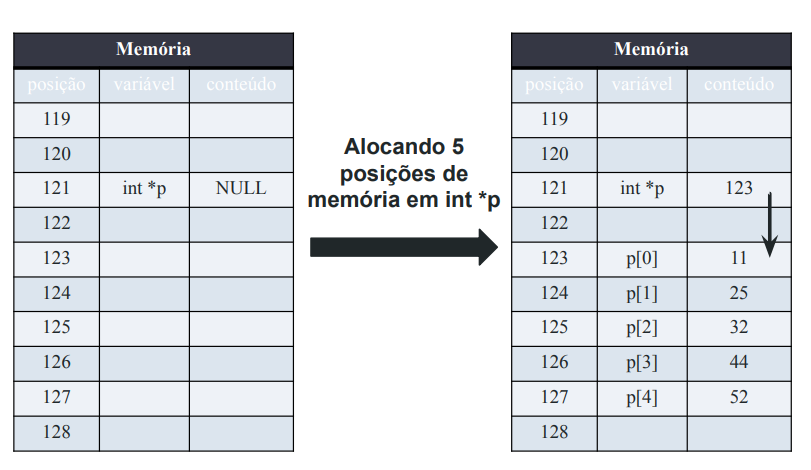
\includegraphics[width=12cm,height=8cm,keepaspectratio=false]{imagens/dynamicaloc.png}
		
	\end{center}
	
	O que acontece acima é que nós temos um pointeiro p que não aponta para nada, aí, usando a alocação dinâmica em tempo de execução no nosso programa, nós alocamos 5 espaços de memória para p. Na prática, é como se estivessemos criando um array (na verdade é extamente isso)
	
	
	\section{Tipos de alocação dinamica}
	
	\subsection{malloc}
	
	\subsubsection{Como funciona?}
	
	A função malloc() serve para alocar memória e tem o seguinte protótipo:
	
	\begin{center}
		\begin{LARGE}
			void *malloc (unsigned int num);
		\end{LARGE}
	\end{center}
	
	Assim, dado o número de bytes que queremos alocar (num), ela aloca na memória e retorna um ponteiro void* para o primeiro byte alocado.
	
	\subsubsection{Exemplo}
	
	Vamos ter um exemplo onde queremos alocar 1000 bytes de memória livre:
	
	\begin{center}
		
		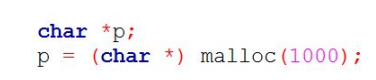
\includegraphics[width=8cm,height=4cm,keepaspectratio=false]{imagens/dynamicaloc2.png}
		
	\end{center}
	
	
	Agora um exemplo vamos alocar espaço de memória para 50 inteiros:
	
	
	\begin{center}
		
		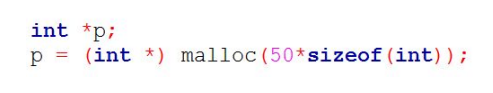
\includegraphics[width=8cm,height=4cm,keepaspectratio=false]{imagens/dynamicaloc3.png}
		
	\end{center}
	
	Uma observação importante é que a função sizeof() cálcula o tamanho do objeto que você passa para ele em bytes, então acima nós calculos o tamanho de um inteiro em bytes e multiplicamos por 50. Além disso, outro detalhe é que se não houver memória suficiente para alocar a memória requisitada,  a função malloc() retorna um ponteiro nulo
	
	\subsection{calloc}
	
	\subsubsection{Como funciona?}
	
	A função calloc() também serve para alocar memória, mas possui um protótipo um pouco
	diferente:
	
	\begin{center}
		\begin{LARGE}
			void *calloc (unsigned int num, unsigned int size)
		\end{LARGE}
	\end{center}
	
	Basicamente, a função calloc() faz o mesmo que a função malloc(). A diferença é que agora
	passamos a quantidade de posições a serem alocadas e o tamanho do tipo de dado alocado
	como parâmetros distintos da função.
	
	\subsubsection{Exemplo}
	
	Vamos ver um exemplo no código a seguir:
	
	\begin{center}
		
		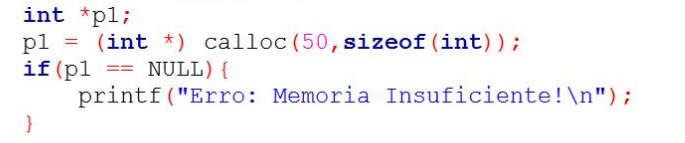
\includegraphics[width=10cm,height=3cm,keepaspectratio=false]{imagens/calloc.png}
		
	\end{center}
	
	Perceba acima que diferentemente do malloc, você passa os parametros de forma distinta (isso pode ser visto separando eles por virgula). Além disso, note o que falamos anteriormente que se não houver memória suficiente para alocar, será retornado um ponteiro nulo
	
	

	
	\subsection{realloc}
	\subsubsection{Como funciona?}
	A função realloc() serve para REALOCAR memória e tem o seguinte protótipo:
	
	\begin{center}
		\begin{LARGE}
			void *realloc (void *ptr, unsigned int num);
		\end{LARGE}
	\end{center}
	
	A função realloc irá modificar o tamanho da memória previamente alocada e apontada por *ptr para o valor indicado por num (sendo que num pode ser maior ou menor do que a quantidade de memória alocada)
	
	Alguns detalhes é que: Se num for 0, a memória apontada por *ptr é liberada (assim como a função free que veremos em breve). Além disso, se *ptr for nulo, o numero de bytes será alocado e devolverá um ponteiro (assim como o malloc faz)
	
	\subsubsection{Exemplo}
	
	Vamos ver um exemplo abaixo com o contexto de um malloc no começo do programa de 5 * sizeof(int)
	
	\begin{center}
		
		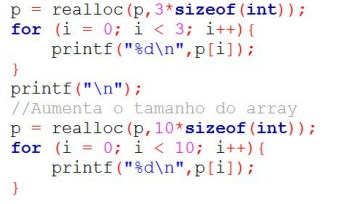
\includegraphics[width=9cm,height=5cm,keepaspectratio=false]{imagens/realloc.png}
		
	\end{center}
	

	
	\subsection{free}
	\subsubsection{Como funciona?}
	
	Quando alocamos memória, nós estamos, na verdade, alocando um array. Ok, isso ja sabemos. Para desalocar essa memória basta utilizar a função free() passando como argumento o ponteiro para a memória alocada. Veja abaixo:
	

	
	
	
	\subsubsection{Exemplo}
	Veja um exemplo abaixo da aplicação disso:
	
	\begin{center}
		
		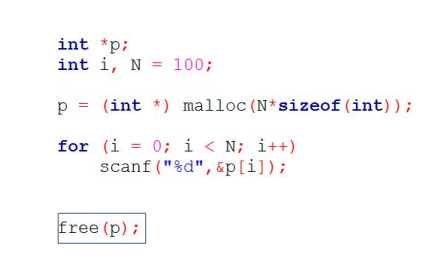
\includegraphics[width=9cm,height=5cm,keepaspectratio=false]{imagens/free.png}
		
	\end{center}
	
	Perceba acima que nós fizemos o alocamento e no final fizemos a liberação
	
	
	
	\section{Casos especiais da alocação dinamica}
	\subsection{Arrays}
	
	\subsubsection{Como funciona?}
	
	Quando temos arrays com mais de uma dimensão, utilizamos o conceito de ponteiro para ponteiro. Veja como esse conceito funciona visualmente:
	
	\begin{center}
		
		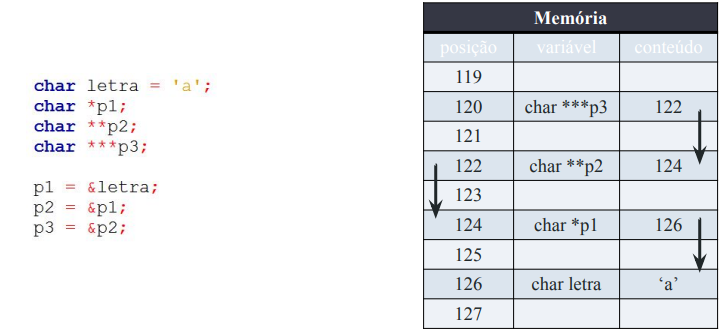
\includegraphics[width=12cm,height=5cm,keepaspectratio=false]{imagens/pointpoint.png}
		
	\end{center}
	
	
	Acima, nós vamos ter a variavel que contém o caractere 'a' e ai vamos ter o ponteiro p1 que aponta para o endereço de memoria dessa variavel, o ponteiro p2 que aponta para o endereco de memoria de p1 e p3 que aponta para o endereço de memória de p2. Se mudamos o endereço de memória que p1 aponta, todo o resto muda.
	
	Entendido isso, veja como funcionará quando queremos alocar memória para um array de mais de uma dimensão (especificamente 2 dimensões):
	
	
	\begin{center}
		
		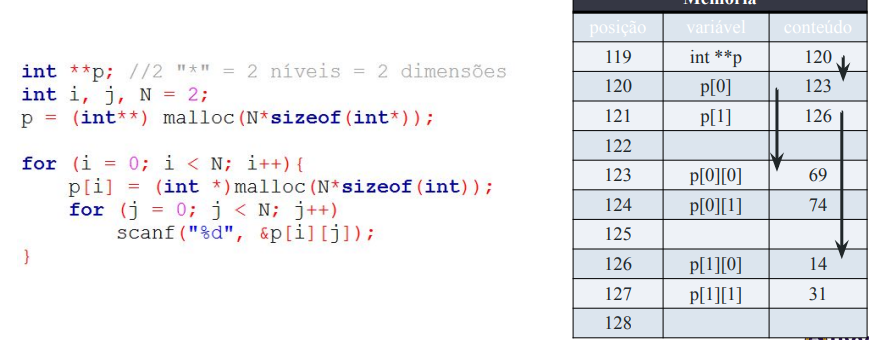
\includegraphics[width=12cm,height=5cm,keepaspectratio=false]{imagens/alocarray.png}
		
	\end{center}
	
	No exemplo acima, o que aconteceu foi:
	
	\begin{enumerate}
		\item int **p;
		\begin{itemize}
			\item Isso declara p como um "ponteiro para um ponteiro de inteiro".
		\end{itemize}
		\item int i, j, N = 2;
		\begin{itemize}
			\item Aqui, declaramos tres variaveis do tipo inteiro. i e j serão utilizadas como contadores nos loops (para percorrer linhas e colunas). A variavel N é definida com o valor 2, o que significa que  
		\end{itemize}
		\item p = (int**) malloc(N*sizeof(int*));
		\begin{itemize}
			\item Esta é a primeira alocação de memória. Utilizando o malloc você está alocando espaço para N ponteiros de inteiro. Assim, p (sendo um ponteiro para ponteiros de inteiro) irá apontar para o bloco de memória p[0] (que é um ponteiro para inteiro) e seguinte ao bloco p[0], temos p[1]. No momento, os ponteiros para inteiros que temos em p[0] e p[1] estão vazios (tecnicamente, apontam para lixo)

		\end{itemize}
		
		\item for (i = 0; i < N; i++) { ... }
		\begin{itemize}
			\item Este é o loop externo. Ele vai ser executado N (2) vezes: uma para i = 0 (primeira linha) e outra para i = 1 (segunda linha).
		\end{itemize}
		
		\item p[i] = (int *)malloc(N*sizeof(int));
		\begin{itemize}
			\item Essa é a segunda alocação de memória. Ela acontece dentro do loop. Nós iremos alocar um espaço na memória para N inteiros.
			\item Quando i = 0, por exemplo, para o ponteiro para inteiros que fica em p[0], ele irá apontar para o endereço de memória onde teremos o nosso primeiro valor e inteiro
		\end{itemize}
		\item for (j = 0; j < N; j++) { ... }
		\begin{itemize}
			\item Este é o loop interno. Ele está aninhado (dentro) do primeiro loop.
			\item Quando i = 0, após p[i] = (int *)malloc(N*sizeof(int)); ter sido executado, p[0] terá um ponteiro que aponta para um endereço de memória que armazena um inteiro e seguido desse endereço, tem um outro endereço de memória que armazena outro inteiro (eles ficam um seguido do outro). Aí que entra o j do loop. Para armazena os inteiros nesse endereço de memória, utilizaremos o j para percorre-los 
			
		\end{itemize}
		\item scanf("\%d", \&p[i][j]);
		\begin{itemize}
			\item scanf é a função que lê dados do teclado
			\item "\%d" diz a ela que esperamos um número inteiro.
			\item \&p[i][j] é onde a mágica acontece:
			\begin{itemize}
				\item Em p[i], estamos acessando o o lugar onde temos o ponteiro para o inteiro, então em p[i][j] estamos acessando o local para onde aquele ponteiro para inteiros aponta. Esse local é o que armazenará o valor do inteiro
				\item O \& (operador "endereço de") passa o endereço exato daquela posição na memória para o scanf, para que ele saiba onde salvar o número que o usuário digitar.
			\end{itemize}
		\end{itemize}
	\end{enumerate}
	
	Veja ainda o processo explicado acima de forma mais visual:
	
		
	\begin{center}
		
		\includegraphics[width=12cm,height=5cm,keepaspectratio=false]{imagens/pointpoint2.png}
		
	\end{center}
	
	\subsubsection{Desalocação}
	
	Agora que já vimos sobre a alocação de memória em arrays de mais de uma dimensão, precisamos ver sobre liberação (desalocamento). Na liberação, ocorre de maneira inversa do alocamento. Nós vamos desalocar a memória primeiro dos ponteiros para inteiros e depois do ponteiro para ponteiros de inteiros. Veja:
	
	\begin{center}
		
		\includegraphics[width=12cm,height=5cm,keepaspectratio=false]{imagens/freepointpoint.png}
		
	\end{center}
	
	
	
	\subsection{Structs}
	
	Assim como nos tipos básicos, também é possível realizar a alocação dinamica de structs.
	
	\subsubsection{Como funciona}
	
	Podemos realizar a alocação de uma única struct ou de mais de uma:
	
	\begin{itemize}
		\item Uma única struct
		\begin{itemize}
			\item Um ponteiro para struct receberá o malloc
			\item Utilizamos o operador seta para acessar o conteúdo
			\item Usamos o free para liberar a memória alocada
		\end{itemize}
	\end{itemize}
	
	
	\begin{center}
	
		\includegraphics[width=10cm,height=5cm,keepaspectratio=false]{imagens/alocstruct1.png}
	
	\end{center}
	
	\begin{itemize}
		\item Mais de uma struct
		\begin{itemize}
			\item Um ponteiro para a struct receberá o malloc
			\item Utilizamos os colchetes para acessar o conteúdo
			\item Usamos o free para liberar a memória alocada	
		\end{itemize} 
	\end{itemize}
	
	\begin{center}
		
		\includegraphics[width=10cm,height=5cm,keepaspectratio=false]{imagens/alocstruct1.png}
		
	\end{center}
	
	\chapter{Listas encadeadas}
	
	\chapter{Pilha e Fila}
	
\end{document}

